% !TEX encoding = UTF-8 Unicode
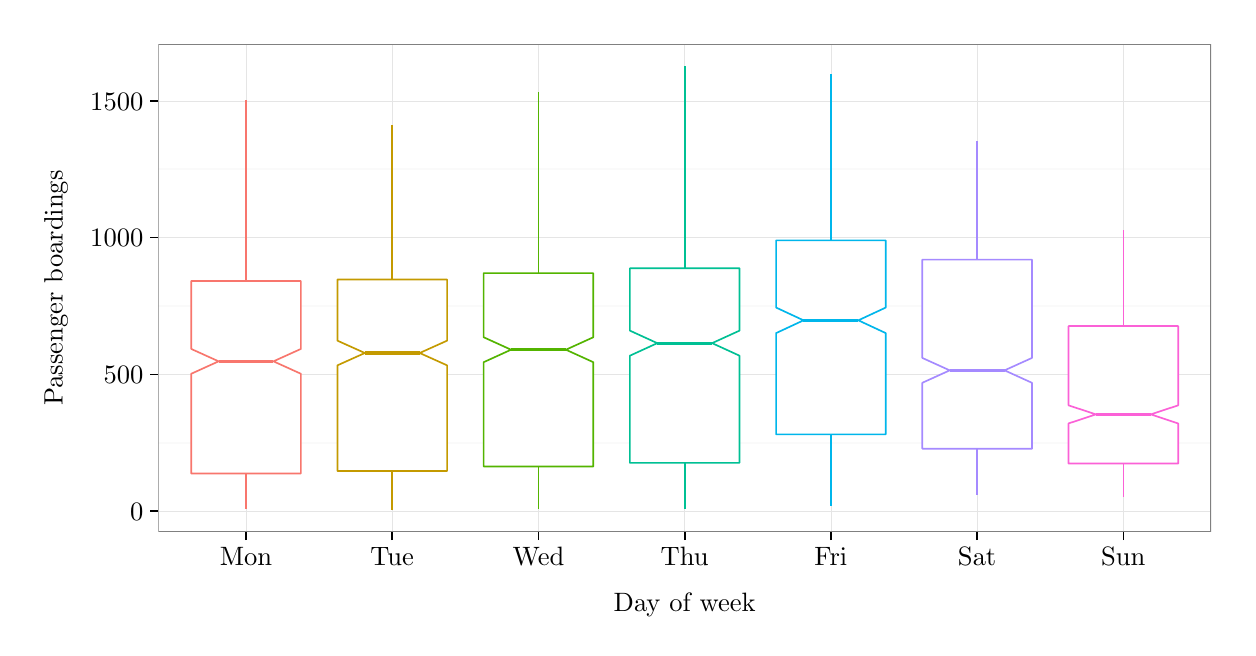
\begin{tikzpicture}[x=1pt,y=1pt]
\definecolor{fillColor}{RGB}{255,255,255}
\path[use as bounding box,fill=fillColor,fill opacity=0.00] (0,0) rectangle (433.62,216.81);
\begin{scope}
\path[clip] (  0.00,  0.00) rectangle (433.62,216.81);
\definecolor{drawColor}{RGB}{255,255,255}
\definecolor{fillColor}{RGB}{255,255,255}

\path[draw=drawColor,line width= 0.6pt,line join=round,line cap=round,fill=fillColor] (  0.00,  0.00) rectangle (433.62,216.81);
\end{scope}
\begin{scope}
\path[clip] ( 47.21, 34.62) rectangle (427.62,210.81);
\definecolor{fillColor}{RGB}{255,255,255}

\path[fill=fillColor] ( 47.21, 34.62) rectangle (427.62,210.81);
\definecolor{drawColor}{gray}{0.98}

\path[draw=drawColor,line width= 0.6pt,line join=round] ( 47.21, 66.84) --
	(427.62, 66.84);

\path[draw=drawColor,line width= 0.6pt,line join=round] ( 47.21,116.24) --
	(427.62,116.24);

\path[draw=drawColor,line width= 0.6pt,line join=round] ( 47.21,165.65) --
	(427.62,165.65);
\definecolor{drawColor}{gray}{0.90}

\path[draw=drawColor,line width= 0.2pt,line join=round] ( 47.21, 42.14) --
	(427.62, 42.14);

\path[draw=drawColor,line width= 0.2pt,line join=round] ( 47.21, 91.54) --
	(427.62, 91.54);

\path[draw=drawColor,line width= 0.2pt,line join=round] ( 47.21,140.95) --
	(427.62,140.95);

\path[draw=drawColor,line width= 0.2pt,line join=round] ( 47.21,190.35) --
	(427.62,190.35);

\path[draw=drawColor,line width= 0.2pt,line join=round] ( 78.91, 34.62) --
	( 78.91,210.81);

\path[draw=drawColor,line width= 0.2pt,line join=round] (131.74, 34.62) --
	(131.74,210.81);

\path[draw=drawColor,line width= 0.2pt,line join=round] (184.58, 34.62) --
	(184.58,210.81);

\path[draw=drawColor,line width= 0.2pt,line join=round] (237.41, 34.62) --
	(237.41,210.81);

\path[draw=drawColor,line width= 0.2pt,line join=round] (290.25, 34.62) --
	(290.25,210.81);

\path[draw=drawColor,line width= 0.2pt,line join=round] (343.08, 34.62) --
	(343.08,210.81);

\path[draw=drawColor,line width= 0.2pt,line join=round] (395.92, 34.62) --
	(395.92,210.81);
\definecolor{drawColor}{RGB}{248,118,109}

\path[draw=drawColor,line width= 0.6pt,line join=round] ( 78.91,125.24) -- ( 78.91,190.85);

\path[draw=drawColor,line width= 0.6pt,line join=round] ( 78.91, 55.72) -- ( 78.91, 42.93);

\path[draw=drawColor,line width= 0.6pt,line join=round,line cap=round,fill=fillColor] ( 59.10,125.24) --
	( 59.10,100.72) --
	( 69.00, 96.24) --
	( 59.10, 91.75) --
	( 59.10, 55.72) --
	( 98.72, 55.72) --
	( 98.72, 91.75) --
	( 88.81, 96.24) --
	( 98.72,100.72) --
	( 98.72,125.24) --
	( 59.10,125.24) --
	cycle;

\path[draw=drawColor,line width= 1.1pt,line join=round] ( 69.00, 96.24) -- ( 88.81, 96.24);
\definecolor{drawColor}{RGB}{196,154,0}

\path[draw=drawColor,line width= 0.6pt,line join=round] (131.74,125.83) -- (131.74,181.76);

\path[draw=drawColor,line width= 0.6pt,line join=round] (131.74, 56.64) -- (131.74, 42.63);

\path[draw=drawColor,line width= 0.6pt,line join=round,line cap=round,fill=fillColor] (111.93,125.83) --
	(111.93,103.71) --
	(121.84, 99.25) --
	(111.93, 94.79) --
	(111.93, 56.64) --
	(151.56, 56.64) --
	(151.56, 94.79) --
	(141.65, 99.25) --
	(151.56,103.71) --
	(151.56,125.83) --
	(111.93,125.83) --
	cycle;

\path[draw=drawColor,line width= 1.1pt,line join=round] (121.84, 99.25) -- (141.65, 99.25);
\definecolor{drawColor}{RGB}{83,180,0}

\path[draw=drawColor,line width= 0.6pt,line join=round] (184.58,128.10) -- (184.58,193.51);

\path[draw=drawColor,line width= 0.6pt,line join=round] (184.58, 58.24) -- (184.58, 42.93);

\path[draw=drawColor,line width= 0.6pt,line join=round,line cap=round,fill=fillColor] (164.77,128.10) --
	(164.77,104.94) --
	(174.67,100.44) --
	(164.77, 95.93) --
	(164.77, 58.24) --
	(204.39, 58.24) --
	(204.39, 95.93) --
	(194.49,100.44) --
	(204.39,104.94) --
	(204.39,128.10) --
	(164.77,128.10) --
	cycle;

\path[draw=drawColor,line width= 1.1pt,line join=round] (174.67,100.44) -- (194.49,100.44);
\definecolor{drawColor}{RGB}{0,192,148}

\path[draw=drawColor,line width= 0.6pt,line join=round] (237.41,129.88) -- (237.41,202.80);

\path[draw=drawColor,line width= 0.6pt,line join=round] (237.41, 59.55) -- (237.41, 43.03);

\path[draw=drawColor,line width= 0.6pt,line join=round,line cap=round,fill=fillColor] (217.60,129.88) --
	(217.60,107.34) --
	(227.51,102.81) --
	(217.60, 98.27) --
	(217.60, 59.55) --
	(257.23, 59.55) --
	(257.23, 98.27) --
	(247.32,102.81) --
	(257.23,107.34) --
	(257.23,129.88) --
	(217.60,129.88) --
	cycle;

\path[draw=drawColor,line width= 1.1pt,line join=round] (227.51,102.81) -- (247.32,102.81);
\definecolor{drawColor}{RGB}{0,182,235}

\path[draw=drawColor,line width= 0.6pt,line join=round] (290.25,139.96) -- (290.25,199.94);

\path[draw=drawColor,line width= 0.6pt,line join=round] (290.25, 69.85) -- (290.25, 44.02);

\path[draw=drawColor,line width= 0.6pt,line join=round,line cap=round,fill=fillColor] (270.44,139.96) --
	(270.44,115.67) --
	(280.34,111.06) --
	(270.44,106.44) --
	(270.44, 69.85) --
	(310.06, 69.85) --
	(310.06,106.44) --
	(300.16,111.06) --
	(310.06,115.67) --
	(310.06,139.96) --
	(270.44,139.96) --
	cycle;

\path[draw=drawColor,line width= 1.1pt,line join=round] (280.34,111.06) -- (300.16,111.06);
\definecolor{drawColor}{RGB}{165,138,255}

\path[draw=drawColor,line width= 0.6pt,line join=round] (343.08,132.99) -- (343.08,175.83);

\path[draw=drawColor,line width= 0.6pt,line join=round] (343.08, 64.67) -- (343.08, 47.87);

\path[draw=drawColor,line width= 0.6pt,line join=round,line cap=round,fill=fillColor] (323.27,132.99) --
	(323.27, 97.47) --
	(333.18, 92.98) --
	(323.27, 88.48) --
	(323.27, 64.67) --
	(362.90, 64.67) --
	(362.90, 88.48) --
	(352.99, 92.98) --
	(362.90, 97.47) --
	(362.90,132.99) --
	(323.27,132.99) --
	cycle;

\path[draw=drawColor,line width= 1.1pt,line join=round] (333.18, 92.98) -- (352.99, 92.98);
\definecolor{drawColor}{RGB}{251,97,215}

\path[draw=drawColor,line width= 0.6pt,line join=round] (395.92,108.98) -- (395.92,143.81);

\path[draw=drawColor,line width= 0.6pt,line join=round] (395.92, 59.31) -- (395.92, 47.18);

\path[draw=drawColor,line width= 0.6pt,line join=round,line cap=round,fill=fillColor] (376.11,108.98) --
	(376.11, 80.34) --
	(386.01, 77.07) --
	(376.11, 73.80) --
	(376.11, 59.31) --
	(415.73, 59.31) --
	(415.73, 73.80) --
	(405.83, 77.07) --
	(415.73, 80.34) --
	(415.73,108.98) --
	(376.11,108.98) --
	cycle;

\path[draw=drawColor,line width= 1.1pt,line join=round] (386.01, 77.07) -- (405.83, 77.07);
\definecolor{drawColor}{gray}{0.50}

\path[draw=drawColor,line width= 0.6pt,line join=round,line cap=round] ( 47.21, 34.62) rectangle (427.62,210.81);
\end{scope}
\begin{scope}
\path[clip] (  0.00,  0.00) rectangle (433.62,216.81);
\definecolor{drawColor}{RGB}{0,0,0}

\node[text=drawColor,anchor=base east,inner sep=0pt, outer sep=0pt, scale=  0.96] at ( 41.81, 38.83) {0};

\node[text=drawColor,anchor=base east,inner sep=0pt, outer sep=0pt, scale=  0.96] at ( 41.81, 88.24) {500};

\node[text=drawColor,anchor=base east,inner sep=0pt, outer sep=0pt, scale=  0.96] at ( 41.81,137.64) {1000};

\node[text=drawColor,anchor=base east,inner sep=0pt, outer sep=0pt, scale=  0.96] at ( 41.81,187.05) {1500};
\end{scope}
\begin{scope}
\path[clip] (  0.00,  0.00) rectangle (433.62,216.81);
\definecolor{drawColor}{RGB}{0,0,0}

\path[draw=drawColor,line width= 0.6pt,line join=round] ( 44.21, 42.14) --
	( 47.21, 42.14);

\path[draw=drawColor,line width= 0.6pt,line join=round] ( 44.21, 91.54) --
	( 47.21, 91.54);

\path[draw=drawColor,line width= 0.6pt,line join=round] ( 44.21,140.95) --
	( 47.21,140.95);

\path[draw=drawColor,line width= 0.6pt,line join=round] ( 44.21,190.35) --
	( 47.21,190.35);
\end{scope}
\begin{scope}
\path[clip] (  0.00,  0.00) rectangle (433.62,216.81);
\definecolor{drawColor}{RGB}{0,0,0}

\path[draw=drawColor,line width= 0.6pt,line join=round] ( 78.91, 31.62) --
	( 78.91, 34.62);

\path[draw=drawColor,line width= 0.6pt,line join=round] (131.74, 31.62) --
	(131.74, 34.62);

\path[draw=drawColor,line width= 0.6pt,line join=round] (184.58, 31.62) --
	(184.58, 34.62);

\path[draw=drawColor,line width= 0.6pt,line join=round] (237.41, 31.62) --
	(237.41, 34.62);

\path[draw=drawColor,line width= 0.6pt,line join=round] (290.25, 31.62) --
	(290.25, 34.62);

\path[draw=drawColor,line width= 0.6pt,line join=round] (343.08, 31.62) --
	(343.08, 34.62);

\path[draw=drawColor,line width= 0.6pt,line join=round] (395.92, 31.62) --
	(395.92, 34.62);
\end{scope}
\begin{scope}
\path[clip] (  0.00,  0.00) rectangle (433.62,216.81);
\definecolor{drawColor}{RGB}{0,0,0}

\node[text=drawColor,anchor=base,inner sep=0pt, outer sep=0pt, scale=  0.96] at ( 78.91, 22.61) {Mon};

\node[text=drawColor,anchor=base,inner sep=0pt, outer sep=0pt, scale=  0.96] at (131.74, 22.61) {Tue};

\node[text=drawColor,anchor=base,inner sep=0pt, outer sep=0pt, scale=  0.96] at (184.58, 22.61) {Wed};

\node[text=drawColor,anchor=base,inner sep=0pt, outer sep=0pt, scale=  0.96] at (237.41, 22.61) {Thu};

\node[text=drawColor,anchor=base,inner sep=0pt, outer sep=0pt, scale=  0.96] at (290.25, 22.61) {Fri};

\node[text=drawColor,anchor=base,inner sep=0pt, outer sep=0pt, scale=  0.96] at (343.08, 22.61) {Sat};

\node[text=drawColor,anchor=base,inner sep=0pt, outer sep=0pt, scale=  0.96] at (395.92, 22.61) {Sun};
\end{scope}
\begin{scope}
\path[clip] (  0.00,  0.00) rectangle (433.62,216.81);
\definecolor{drawColor}{RGB}{0,0,0}

\node[text=drawColor,anchor=base,inner sep=0pt, outer sep=0pt, scale=  0.96] at (237.41,  6.00) {Day of week};
\end{scope}
\begin{scope}
\path[clip] (  0.00,  0.00) rectangle (433.62,216.81);
\definecolor{drawColor}{RGB}{0,0,0}

\node[text=drawColor,rotate= 90.00,anchor=base,inner sep=0pt, outer sep=0pt, scale=  0.96] at ( 12.61,122.72) {Passenger boardings};
\end{scope}
\end{tikzpicture}
